\subsubsection{问题一的模型建立}
由式 \eqref{eq:event-expansion} 得到计划 \(i\) 的完整事件集合 \(E_i\)。按假设（1）统一采用半开区间，记其频段区间为 \(F_i=[f_i^-,f_i^+)\)。对于任意两个不同计划 \(i,j\)，当且仅当频段区间相交且至少存在一对重复事件的时间区间相交时，将二者记为冲突装备对：
\begin{equation}
C_{ij}=
\begin{cases}
1, & F_i\cap F_j\ne\varnothing,\ 
\exists k,\ell:\ I_{ik}\cap I_{j\ell}\ne\varnothing,\\
0, & \text{otherwise}.
\end{cases}
\label{eq:q1-conflict}
\end{equation}
同一装备对即使对应多次事件重叠，也只在冲突清单中保留一条边；事件级重叠次数另行统计，用于核对检测结果而不替代装备对数量。

\subsubsection{问题一的求解}
采用完整枚举而不是只比较首次使用区间。计算流程为：先筛选频段区间不相交的计划对，再对剩余计划对展开事件区间并进行半开区间相交判断；一旦发现一对时频同时相交的事件，就记录该装备对并停止对该对的重复计数。随后利用离散时频资源格倒排索引重新生成冲突对，作为独立复核。

\subsubsection{问题一的结果}
150 条计划展开为 1,300 个重复事件，共检查 \(C(150,2)=11\,175\) 个候选装备对，得到 297 对冲突装备，占候选装备对的 2.66%。这些装备对对应 431 次事件级重叠，因此“冲突装备对数”和“事件重叠次数”分别回答了计划层和事件层两个不同问题。

冲突边的类别结构见图 \ref{fig:q1-matrix}。图中每个方格表示一对计划是否至少出现过一次时频同时相交；同一对的多次事件重叠不重复增加方格。B--C 类边用独立的强调色标出，便于观察冲突集中区域，但颜色只承担类别提示，精确数量仍以表 \ref{tab:q1-category} 为准。

\begin{figure}[htbp]
  \centering
  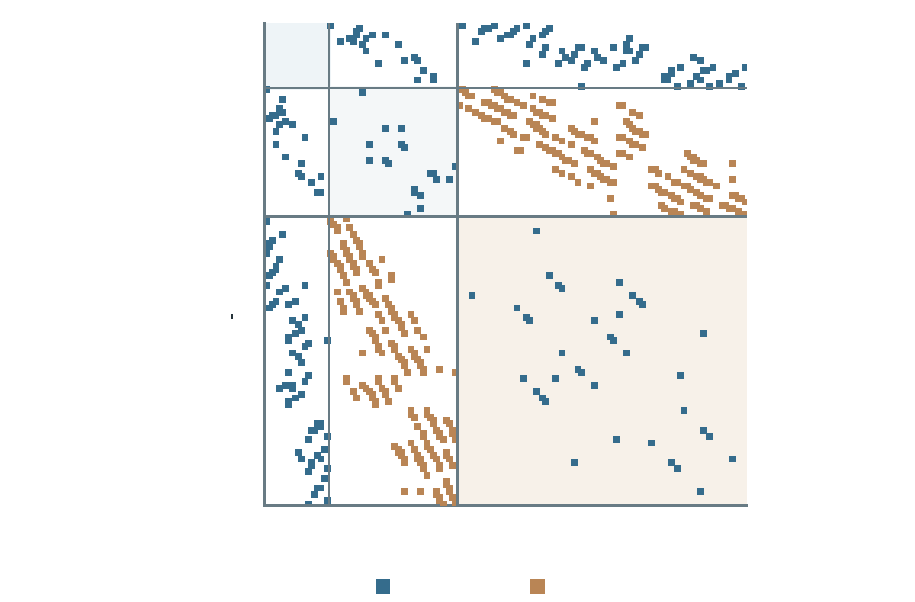
\includegraphics[width=0.86\textwidth]{figures/fig2_q1_conflict_matrix.pdf}
  \caption{问题一计划层冲突矩阵}
  \label{fig:q1-matrix}
\end{figure}

\begin{table}[H]
\centering
\caption{问题一按类别组合统计的冲突结果}
\label{tab:q1-category}
\begin{tabular}{lrrrr}
\toprule
类别组合 & 可配对数 & 冲突对数 & 类别内冲突率 & 占全部冲突对 \\
\midrule
A--A & 190 & 0 & 0.00\% & 0.00\% \\
A--B & 800 & 21 & 2.63\% & 7.07\% \\
A--C & 1\,800 & 66 & 3.67\% & 22.22\% \\
B--B & 780 & 10 & 1.28\% & 3.37\% \\
B--C & 3\,600 & 181 & 5.03\% & 60.94\% \\
C--C & 4\,005 & 19 & 0.47\% & 6.40\% \\
\midrule
合计 & 11\,175 & 297 & -- & 100.00\% \\
\bottomrule
\end{tabular}
\end{table}

表 \ref{tab:q1-category} 显示，B--C 类既贡献了最多的冲突装备对，按全部可能配对归一化后冲突率也最高。这个结果用于说明冲突结构和后续优化的输入重点，不直接规定问题二中应该移动或撤销哪些计划。

\subsubsection{问题一的检验}
独立离散资源格算法得到的 297 对冲突装备与连续半开区间算法完全一致；重新枚举事件矩形交集得到 431 次事件级重叠，与主程序一致。A001 第二次使用事件和 C083 最后一次使用事件分别通过示例语义和边界复核。输出工作簿保留附件模板的单工作表和三列字段，297 行结果与 \texttt{results.json}、\texttt{conflict\_pairs.csv} 逐行一致。

\subsubsection{问题一小结}
问题一得到的 297 条冲突边构成问题二的硬约束输入；其后的冲突消解必须重新展开每个调整动作的全部重复事件，不能只对首次事件进行局部修复。
